\documentclass[a4paper,10pt]{article}
\usepackage{fullpage}
\usepackage{times}
\usepackage{upquote}
\usepackage{url}
\usepackage[tikz]{bclogo}
\usepackage{graphicx}
\usepackage{float}

\graphicspath{ {images/} }


\def\signed #1{{\leavevmode\unskip\nobreak\hfil\penalty50\hskip2em
  \hbox{}\nobreak\hfil(#1)%
  \parfillskip=0pt \finalhyphendemerits=0 \endgraf}}

\newsavebox\mybox
\newenvironment{aquote}[1]
  {\savebox\mybox{#1}\begin{quote}}
  {\signed{\usebox\mybox}\end{quote}}


\newcommand{\code}[1]{\texttt{\small #1}}

\newcommand*{\TakeFourierOrnament}[1]{{%
\fontencoding{U}\fontfamily{futs}\selectfont\char#1}}
\newcommand*{\danger}{\TakeFourierOrnament{66}}

\begin{document}

\title{L41: Lab Setup}
\author{Dr Robert N.~M. Watson \and Dr Graeme Jenkinson}
\date{2019-2020}
\maketitle

L41 is taught through a blend of lectures and laboratory experiments.
The purpose of the labs is threefold: to teach you about real-world operating
systems, to teach you experimental methodology and practical skills, and to
provide fodder for assessment.
You will use tools such as DTrace to explore the behaviour of the system
through `potted' example programs that will trigger OS behaviours for you to
investigate.
Each lab is structured as a set of mandatory experimental questions; take care
to ensure that your lab report addresses all of the assigned experimental
questions.

\section*{Experimental platform}

Our experimental platform is the open-source FreeBSD operating system running
on the BeagleBone Black (BBB) board, described in the remainder of this
handout.

\subsection*{The operating system: FreeBSD}

We will be using the open-source FreeBSD operating system's ARMv7 port on the
BeagleBone Black.
FreeBSD is of particular interest due to its tight integration of a number of
tracing and measurement tools (e.g., DTrace) and that it is built by default
with the Clang/LLVM compiler suite, which make it easier to insert additional
instrumentation.
You can learn more about FreeBSD by visiting the FreeBSD Project's website:

\smallskip
\url{https://www.FreeBSD.org/}
\smallskip

The course text, \textit{The Design and Implementation of the FreeBSD
Operating System, Second Edition} will be a useful reference, covering
concepts such as the process model, inter-process communications, and
filesystems.
There is also a section on the implementation of DTrace, which may be useful
background material for the labs.
\textit{DTrace: Dynamic Tracing in Oracle Solaris, Mac OS X and FreeBSD} is a
detailed, user-facing guide on how to use DTrace, and will also be a useful
reference for the labs.

\subsection*{The board: BeagleBone Black}

The BeagleBone Black board is based on a Texas Instruments System on Chip that
employs a single-core ARM Cortex-A8 processor; it includes on-board flash, an
Ethernet MAC, USB support, and an SD Card slot.
This 32-bit processor is not the zippiest in the world -- but it is widely
deployed and fully functional with respect to many of the behaviours of
interest for this course, including having processor performance counters.
In our configuration, FreeBSD boots from the on-board SD Card.

We will access the board as a USB device from lab workstations or personal
notebook computers.
``USB target mode'' allows the BBB to appear to be a set of USB devices to the
attached workstation: an Ethernet device that can be used to SSH into the
board, and a USB device that accesses a serial console.
Power is also provided using the USB cable.
These instructions describe how to access the board from a Linux workstation
in the lab.
Other configurations, such as Mac or Windows notebooks, or FreeBSD
workstations, may also work with suitable adjustment to client-side tools.

While the BBB is not enormously expensive, they are often back ordered, so
acquiring replacements can be inconvenient.
If you lose or damage your board (e.g., by dropping it), then we may ask you
to pay to replace the board.
It is fairly straight forward to ``brick'' the board by overwriting the
contents of its on-board flash, the OS image on the SD Card, etc.; this is
discouraged.
If this appears to have occurred, please contact the module instructor for
assistance.
A small number of replacement boards are available if required.

It is easy to replace the SD Card in the board -- should it appear to have
become corrupted or entered an unusable state (they appear to be sensitive to
power being removed from the device while an operation is in progress), let us
know and we can provide a replacement.
Note that any customisation to your board (e.g., SSH keys, \code{/data}
partition) will not be present on the replacement card -- do ensure that you
keep the primary copy of any important data on your workstation.

\subsection*{Getting started}

The BeagleBone Black will arrive in a compact plastic case, and with a
pre-initialised SD Card holding the OS image.
For the purposes of this course, you should not need to disassemble the case
or eject the card, except to install an image upgrade that might be provided
by the instructors.
We will power and communicate with the board via a single USB cable.
These directions assume that you will be working on an ACS Workstation running
Ubuntu Linux.
However, our teaching setup has also been used with varying degrees of success
with other systems, including FreeBSD and Mac OS X\footnote{We have had mixed
experience with Mac OS X and Windows, as the OS image on the BBB implements
`USB target mode' -- i.e., appears to be a set of USB devices -- and device
drivers on operating systems vary quite a bit.
If you appear to have reliability problems with the serial console or Ethernet
parts, it may well be a device-driver bug.
You are welcome to help us debug the problem, but it may be simpler to work
with the systems that we have tested with.}.
The BBB appears to the workstation operating system as two USB devices: a USB
serial port, which reaches a console, and a USB Ethernet device, which can be
used to SSH into the OS instance on the board.

%When you plug in the BeagleBone Black, at least one blue LED should light up
%on the board.
%It can take a minute or so for the OS image to boot; once it does, the two USB 
%devices will become visible on the workstation.
%You can connect to the console using the following command:

%\begin{small}
%\begin{verbatim}
%$ minicom -o -D /dev/ttyACM0
%\end{verbatim}
%\end{small}

When you plug in the BeagleBone Black, at least one blue LED should light up
on the board.
It can take a minute or so for the OS image to boot. Once booted, two USB
devices will become visible on the workstatation. You can then connect to the 
console using the following command:

\begin{small}
\begin{verbatim}
$ minicom -o -D /dev/ttyACM0 115200
\end{verbatim}
\end{small}

You should be able to log in as \code{root} without a password. In order
to stream data or copy files to and from the board, it is preferable to 
login to the board using SSH.
To do this, you will first need download a \textbf{insecure} private key:

\smallskip
\noindent
{\small
\url{https://www.cl.cam.ac.uk/teaching/1920/L41/private/2019-2020-l41-insecure-private-key}
}
\smallskip

Once downloaded, copy the file to you \code{\textasciitilde/.ssh} directory on
your workstation (ensuring that the correct permissions \code{chmod 0600
2019-2020-l41-insecure-private-key} are set).  To simplify key management your
may wish to add the following configuration into your SSH config file
(\code{\textasciitilde/.ssh/config}):

\begin{small}
\begin{verbatim}
Host 192.168.141.100
    IdentityFile ~/.ssh/2019-2020-l41-insecure-private-key
\end{verbatim}
\end{small}

Once the key is installed, you should be able to login to the BBB through SSH:

\begin{small}
\begin{verbatim}
$ ssh root@192.168.141.100
\end{verbatim}
\end{small}

\begin{bclogo}[logo=\bcattention, noborder=true, barre=none]{Important!}
    The key pair used to provide SSH access to the BBB are the moral
    equivalent of a default password known to the world.  \textbf{DO NOT} use
    this key pair for any other purpose.
\end{bclogo}


\begin{bclogo}[logo=\bcattention, noborder=true, barre=none]{Important!}
    When running as \code{root}, you should exercise caution: accidentally
    deleting system files may (will) render your board unbootable or cause loss
    of your scripts or data.
\end{bclogo}

Now, run your first DTrace script:

\begin{small}
\begin{verbatim}
# cd /data
# dtrace -qn 'BEGIN { printf("Hello world"); exit(0); }'
\end{verbatim}
\end{small}

To write the output of a script to a file, you can redirect standard output to
a file:

\begin{small}
\begin{verbatim}
# dtrace -qn 'BEGIN { printf("Hello world"); exit(0); }' > data.out
\end{verbatim}
\end{small}

We have configured the root filesystem to be read-only by default, in order to
reduce the chance of accidents, but also to reduce wear on the SD Card.
The \code{/data} filesystem is writable, however, and is a good place to stick
your scripts, data, compiler output, etc., so that it will persist across
reboots.
You will likely wish to copy files from the BeagleBone Black to your
workstation for analysis -- e.g., to load it into a spreadsheet.
You may also want to edit scripts and source files on the workstation.
You can copy files back and forth using \code{scp}; for example, this command
can be run on the ACS Workstation to copy \code{data.out} to your current
working directory:

\begin{small}
\begin{verbatim}
$ scp root@192.168.141.100:/data/data.out .
\end{verbatim}
\end{small}

%\subsection*{Connecting to the TTL serial console}
%
%Although it is unlikely you will require access to the boot console, this can
%be done via a FTDI-to-TTL adapter available from the module instructor.
%The three pins should be labeled and connected as follows:
%
%\medskip
%\begin{tabular}{llll}
%\hline
%  Colour & Label & Function & Pin \\
%\hline
%  Black & GND & Ground & 1 \\
%  Red & TXD & Transmit Data & 4 \\
%  Green & RCD & Receive Data & 5 \\
%\hline
%\end{tabular}
%\medskip
%
%\noindent
%These should be connected to 6-pin serial block on the BeagleBone Black.
%Pin 1 has a white dot next to it.
%The default TTL console speed is 115,200 bps; attempting other speeds may
%interrupt the boot or trigger a serial break to the kernel debugger.
%

\subsection*{Running the Jupyter notebook}

To start the Jupyter Notebook \code{ssh} to the BeagleBone Black (\code{ssh
root@192.168.141.100}) and run the \code{jupyter} command as follows (note
that the \code{jupyter} command must be run as \code{root} so that the notebook
 has permission to execute DTrace scripts):

\begin{small}
\begin{verbatim}
# cd /data
# jupyter notebook
\end{verbatim}
\end{small}

On starting, the Jupyter Notebook prints the address on which it can be
accessed with a Web browser; this should be
\texttt{http://192.168.141.100:8888} (this can take several seconds to
appear so please be patient)\footnote{The ``Widgets are unavailable'' is
benign and may be ignored.}.  From the ACS Workstation open a Web browser
at this address.  The Jupyter dashboard should then be shown:

\begin{figure}[H]
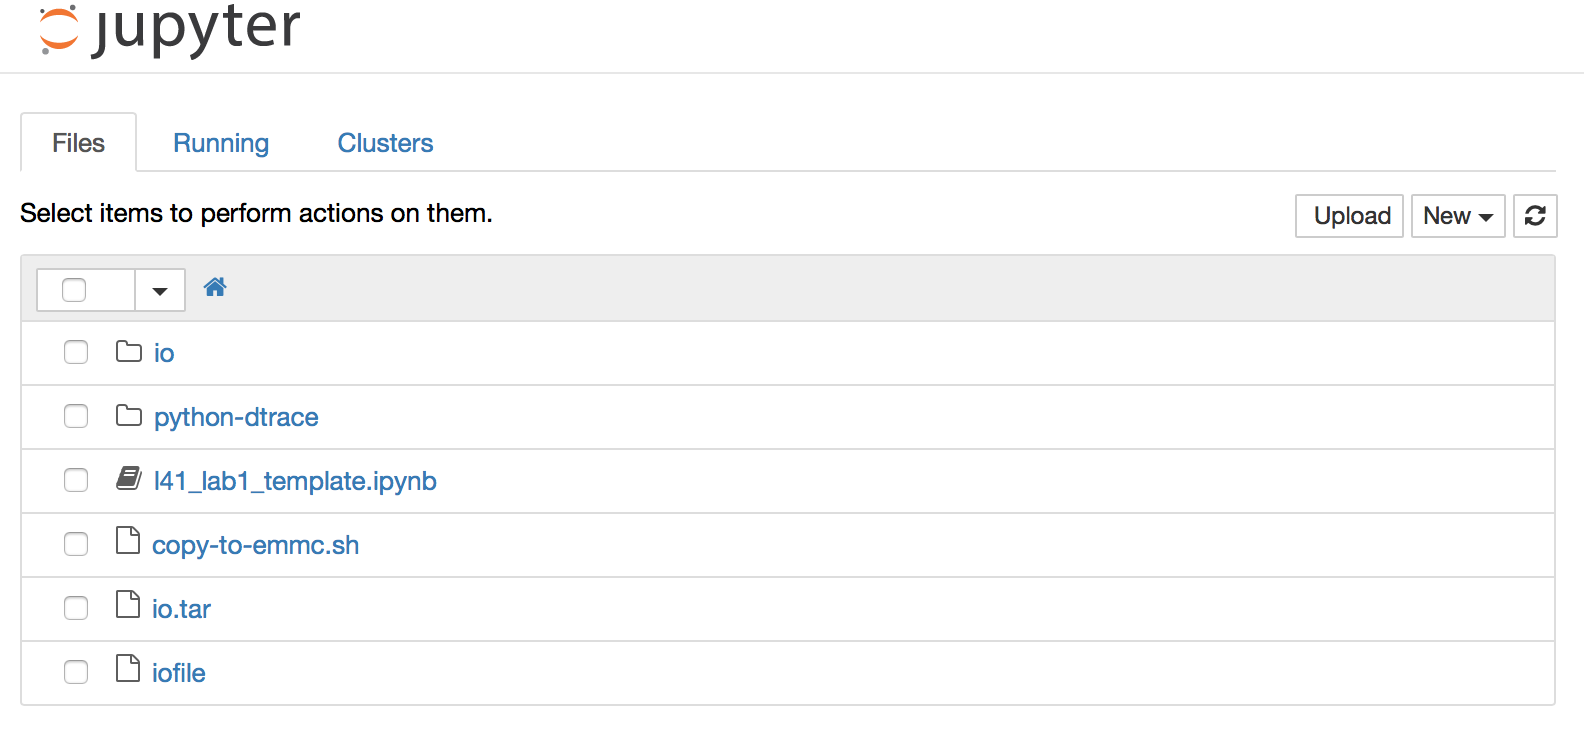
\includegraphics[width=\linewidth]{jupyter_home.png}
\end{figure}

Jupyter (formerly IPython) Notebooks are identified by the file extension
\code{.ipynb}. To open a Notebook simply click on its name. The selected
Notebook will open in a separate tab from which it can be edited and run.

\subsubsection*{Running the benchmarks}

Within a Jupyter notebook (residing in the BBB's \code{/data} directory) the
I/O benchmarks ({\code{io-static} and \code{io-dynamic}) can be run as
follows\footnote{Note \code{!} is a Jupyter ``magic'' for executing running
shell commands.}:

\begin{figure}[H]
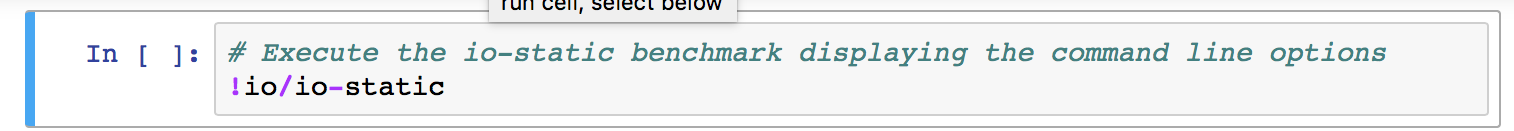
\includegraphics[width=\linewidth]{jupyter_running_benchmark.png}
\end{figure}

To execute a cell (in this instance to run the benchmark), simply select it and
then press the ``run cell'' button in the Jupyter Notebook toolbar:

\begin{figure}[H]
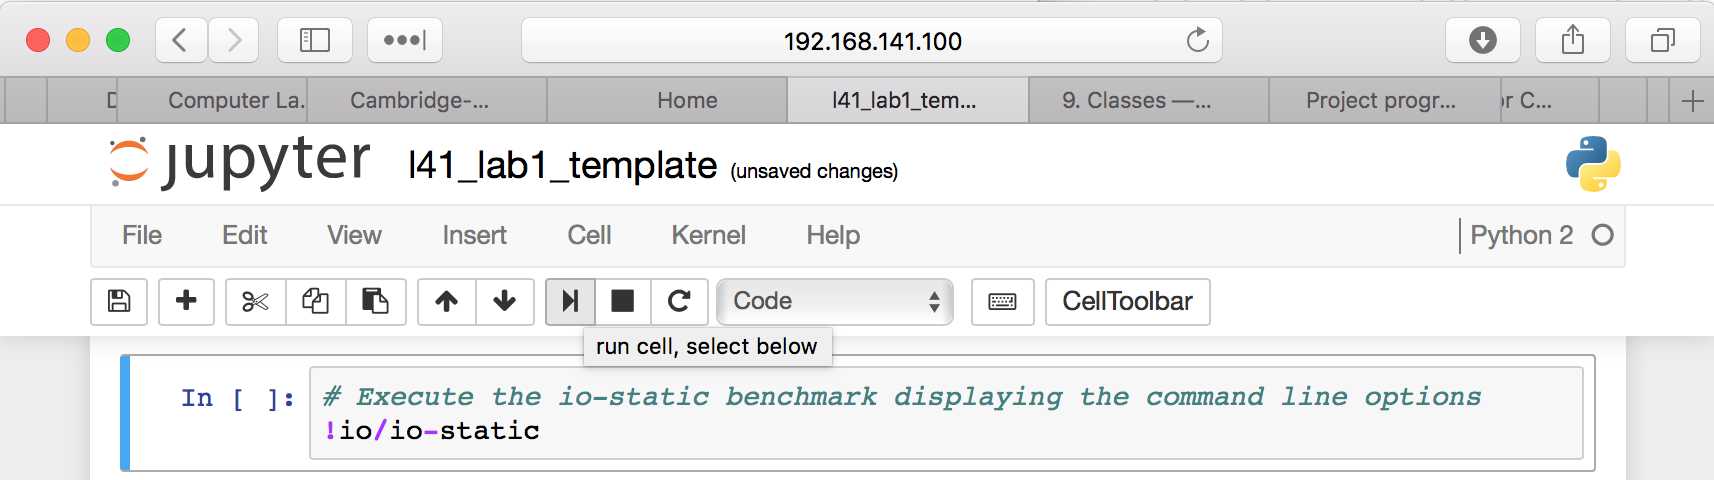
\includegraphics[width=\linewidth]{jupyter_run_cell.png}
\end{figure}

The Jupyter Notebooks used for the L41 laboratories use a Python kernel running
on the BBB. This allows Python scripts and Jupyter shell commands
(such as those used to invoke the benchmarks) to be freely intermixed. This 
allows, for example, running the benchmark in a loop where each
iteration uses a different set of parameters:

\begin{figure}[H]
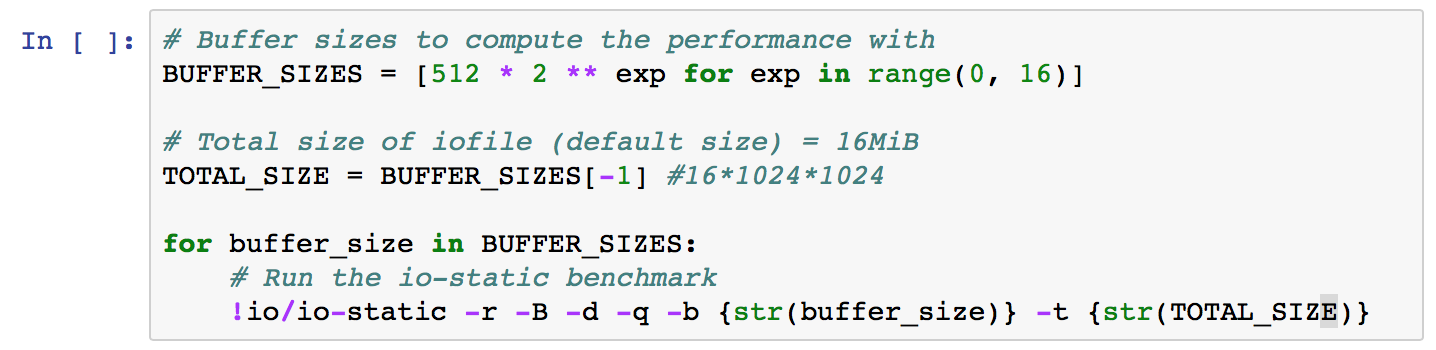
\includegraphics[width=\linewidth]{jupyter_running_benchmark_loop.png}
\end{figure}

The output of a shell command can be captured into a Python variable (an array
with an entry for each row of the output) as follows:

\begin{figure}[H]
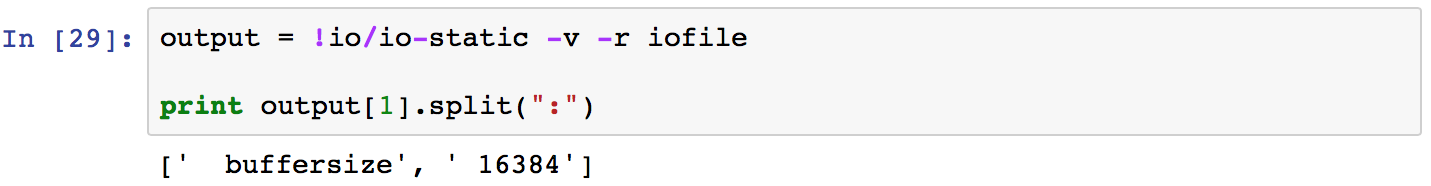
\includegraphics[width=\linewidth]{jupyter_running_benchmark_capture.png}
\end{figure}

\subsubsection*{Running DTrace scripts}

DTrace scripts can be executed within the Jupyter notebook with the assistance
of the \code{python-dtrace} module. In order to run the I/O benchmark and
also instrument it with DTrace, scripts are executed within a separate thread
by instantiating a \code{DTraceConsumerThread} object. The
\code{DTraceConsumerThread} constructor takes a Python string specifying
D-Language script to execute, as well as several other optional parameters. In
the example shown below, the script uses a DTrace aggregation to count the
number of sycalls invoked by the I/O benchmark. The
\code{DTraceConsumerThread} instance is constructed with the
\code{walk\_func} parameter. This callback is invoked periodically with the
current value of the aggregation reported by the kernel; in this example the
callback stores the total value of the aggregation within a Python dictionary.

\begin{figure}[H]
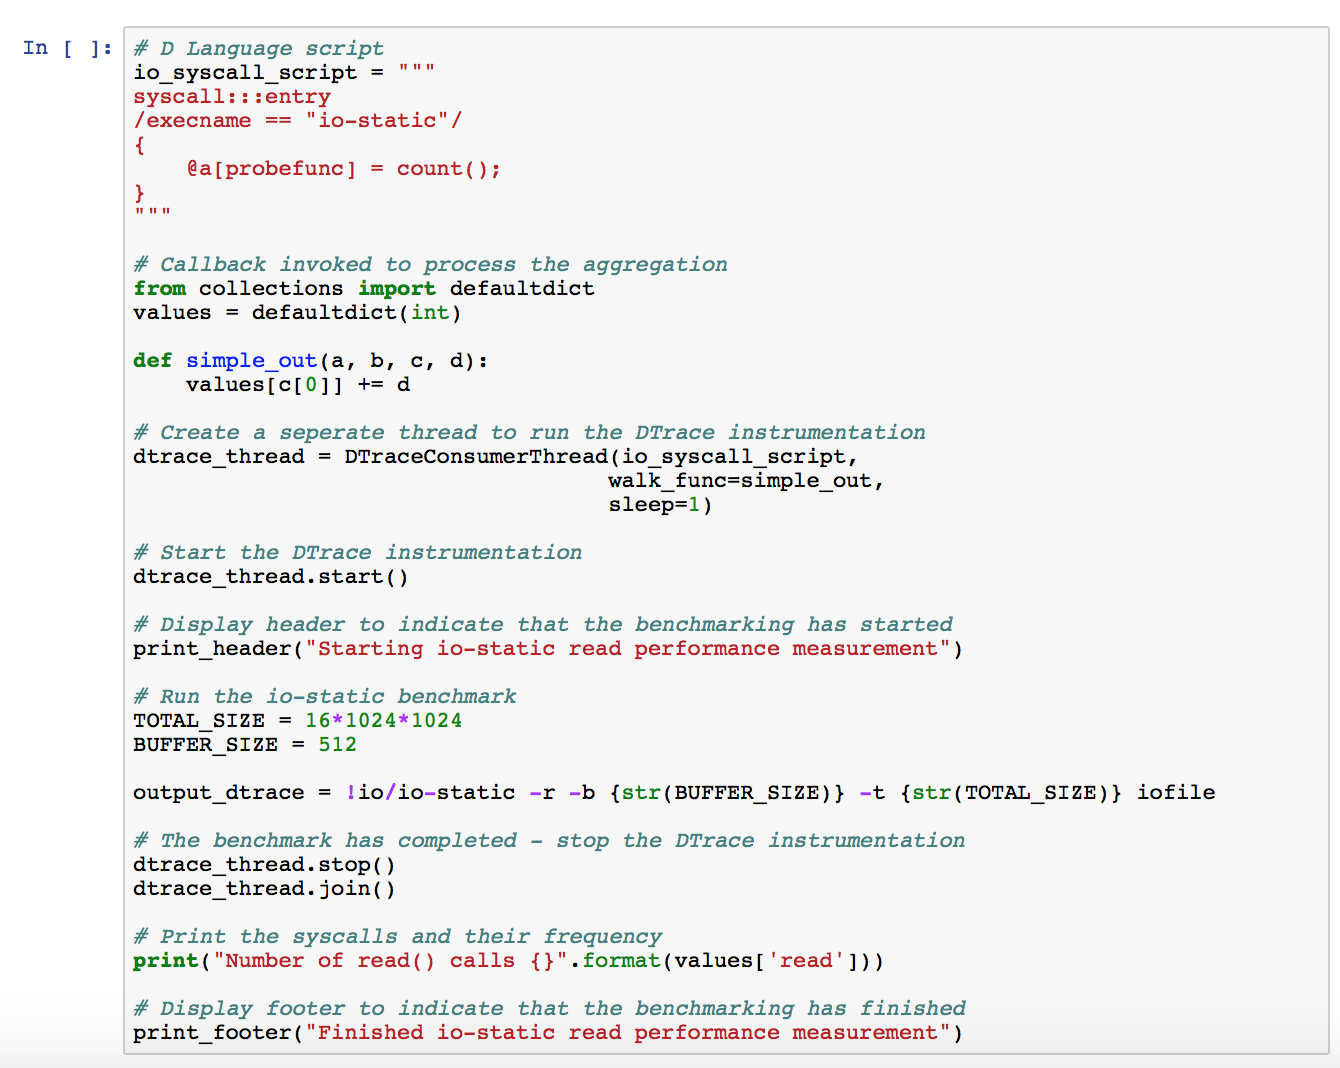
\includegraphics[width=\linewidth]{jupyter_python_dtrace.png}
\end{figure}

Similarly, a \code{DTraceConsumerThread} can be constructed specifying the
\code{out\_func} parameter. This specifies a callback that is invoked by
DTrace when a \code{print}-like action is processed. The Jupyter notebook
template for first laboratory provides a example of how this may be used.

\subsubsection*{Plotting performance measurements}

Performance measurements can be plotted inside the Jupyter Notebook using the
built-in ``magic'': \code{\%matplotlib inline}.  A simple example, plotting a
sine waveform, is given below:

\begin{figure}[H]
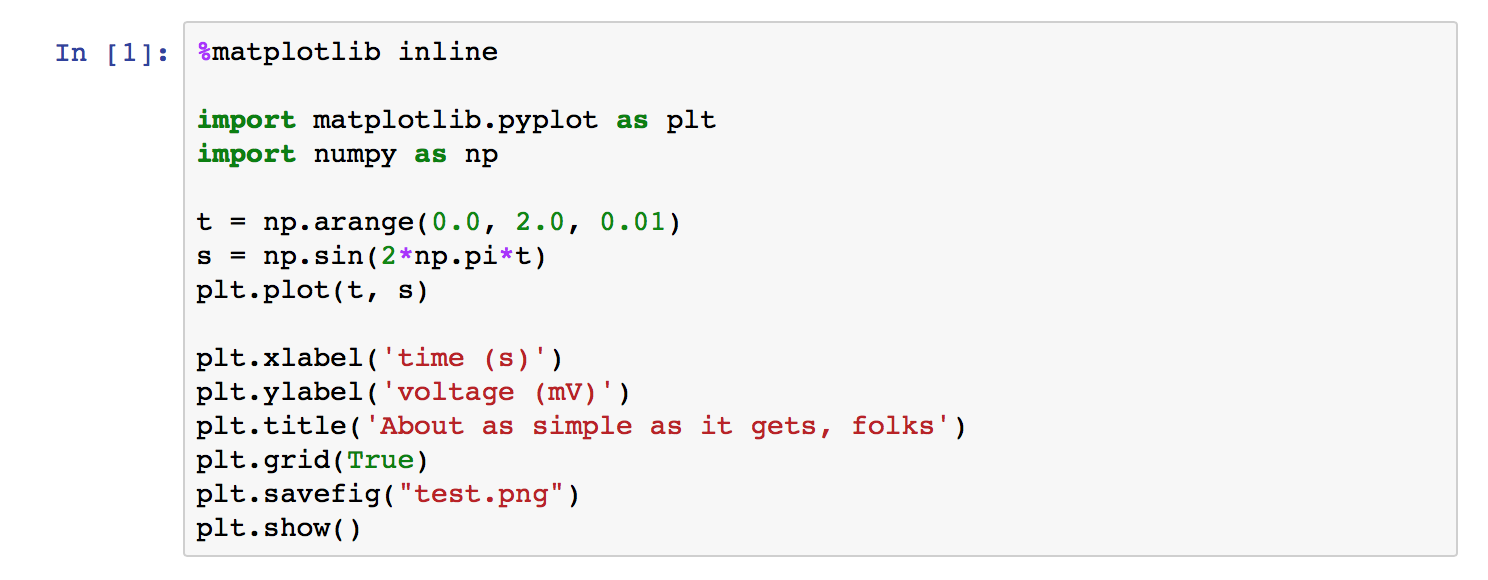
\includegraphics[width=\linewidth]{jupyter_matplotlib.png}
\end{figure}

In addition to displaying inline, matplotlib graphs can be saved to the BBB
filesystem using the \code{plt.savefig()} function. Saved files can then be
copied from the BBB to the ACS Workstation using \code{scp} for inclusion in
your laboratory reports:

\begin{small}
\begin{verbatim}
$ scp root@192.168.141.100:/data/test.png .
\end{verbatim}
\end{small}

Further information about matplotlib can be found at the project's website:
\url{matplotlib.org}.

\subsubsection*{Analysing performance measurements}

\begin{aquote}{\url{pandas.pydata.org}}
pandas is an open source, BSD-licensed library providing high-performance,
easy-to-use data structures and data analysis tools for the Python programming
language.
\end{aquote}

In this laboratory, performance measurements capture how the \textit{dependent
variable} (I/O read and write bandwidth) changes as a result to changes in the
\textit{independent variable} (for example, buffer size).  This data is best
represented in pandas using a \code{DataFrame}. The pandas \code{DataFrame} is
a tabular structure comprised of rows and columns. A \code{DataFrame} can be
used to, for example, store the performance of a benchmark with the rows
representing runs of the benchmark for different buffer sizes. And the columns
of the \code{DataFrame} representing repeated runs of the benchmark for a given
buffer size. 

A flat list a performance values can be converted into a n-by-m array for
loading into a \code{DataFrame} using the Python module \code{numpy}'s
reshape function:

\begin{figure}[H]
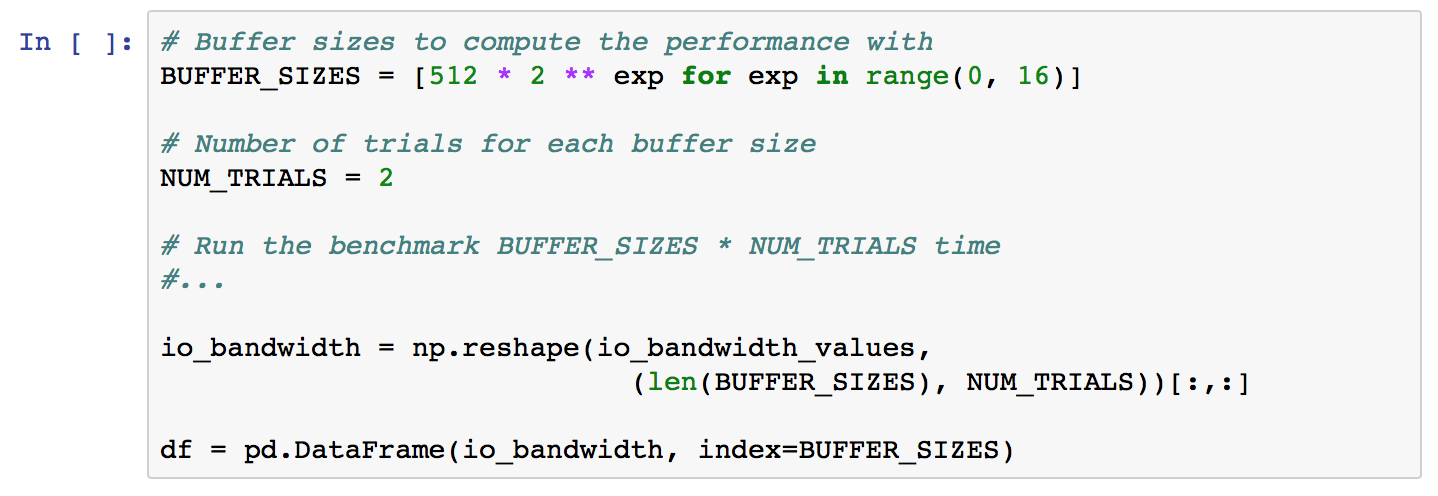
\includegraphics[width=\linewidth]{jupyter_pandas.png}
\end{figure}

Once a \code{DataFrame} has been created, statistics such as the median or
the 25 and 75 percentile values can be computed directly:

\begin{small}
\begin{verbatim}
df.median(1) # Median value of rows
df.quartile([.25, .75], axis=1) # 25th and 75th quartile value of rows
\end{verbatim}
\end{small}

Further information about pandas can be found at the project's website:
\url{pandas.pydata.org}.

\subsection*{Troubleshooting}

In the event of the Jupyter Notebook behaving erratically the first port of
call is to simply stop the currently executing cell (this can be done from the
Jupyter Notebook toolbar). For more serious problems (such as systemic
unresponsiveness) the executing ``kernel'' can be reset from the Jupyter
toolbar. This resets the Python runtime's state and is an effective for most
problems. If resetting the kernel does not resolve the issue it may be to
terminate and restart the \code{jupyter} command.

As a fallback, it is acceptable to complete the laboratory without using 
Jupyter Notebooks. Instructions for completing the laboratories using
only tools available from the shell can be found in 
the 2015-16 interation of the course materials:

\smallskip
\url{https://www.cl.cam.ac.uk/teaching/1516/L41/materials.html}
\smallskip

\subsection*{Shutting down}

Simply powering off the BeagleBone Black (e.g., by unplugging it) will be
harmless in most situations, but could lead to data loss.
It is preferable to instead first run \code{shutdown -p now} to initiate a
software poweroff.
Once the system has shut down, the blue LED will turn off, and it is safe to
unplug the board.

\end{document}
